\chapter{Conclusão}
\label{cha:conclusao}
\index{Conclusão}
% ============================================================
% CONCLUSÃO ATUALIZADA — TCC
% Calibração Multivariada: RLM com Métodos de Conjunto
% ============================================================
%
% MUDANÇAS EM RELAÇÃO À CONCLUSÃO ORIGINAL:
%
% 1. Inverteu o vencedor para Mn, Cr e Ni:
%    - Mn: RLM clássica → RLM-subagging
%    - Cr: ensemble → RLM clássica
%    - Ni: RLM clássica → RLM-subagging (marginal)
%
% 2. Corrigiu os valores numéricos de tempo:
%    - "2,5 vezes" → 3,0 vezes
%    - "15 a 20 vezes" → "até 19 vezes" (faixa 3x–19x)
%
% 3. Acrescentou o protocolo de CV 5-fold como contribuição
%    metodológica do trabalho
%
% 4. Acrescentou MAE e R² como métricas adicionais e o
%    conceito de dominância de Pareto para Mn e Ni
%
% 5. Removeu afirmações sobre Cr e Fe como os beneficiados
%    únicos pelos métodos de ensemble
% ============================================================

\begin{comment}

Este estudo realiza uma investigação sistemática das técnicas de
reamostragem \textit{bootstrap}, \textit{bagging} e
\textit{subagging}, aplicadas à Regressão Linear Múltipla (RLM) no
contexto de calibração multivariada de dados oriundos de amostras de
aço-ligas, atendendo integralmente aos objetivos propostos. As
abordagens foram implementadas com sucesso utilizando a RLM como
modelo base, e os experimentos foram conduzidos com protocolo
metodologicamente controlado --- incluindo otimização de parâmetros
por validação cruzada 5-\textit{fold} aplicada exclusivamente ao
conjunto de calibração ---, garantindo comparações justas e
reprodutíveis entre os algoritmos \textit{RLM clássica},
\textit{RLM-bagging} e \textit{RLM-subagging}. Além do RMSEP, as
métricas \gls{MAE} e R$^2$ foram incorporadas à análise, ampliando a
caracterização do desempenho preditivo de cada técnica.

A análise comparativa entre os algoritmos revela variações de
desempenho dependentes do analito avaliado, confirmando a inexistência
de uma técnica universalmente superior. Para o Manganês (Mn), o
RLM-\textit{subagging} ($k^* = 80\%$, $m^* = 10$) apresentou o
menor RMSEP (0,0966), representando uma redução de 8,1\% em relação à
RLM clássica. Para o Ferro (Fe), o RLM-\textit{bagging} ($m^* = 30$)
obteve o melhor desempenho (RMSEP~=~2,6406), com melhoria de 4,0\%
sobre a RLM clássica. Para o Níquel (Ni), o RLM-\textit{subagging}
($k^* = 60\%$, $m^* = 10$) apresentou resultado marginalmente superior
(RMSEP~=~1,6003), com diferença de 0,25\% em relação à RLM clássica.
Em contrapartida, para o Molibdênio (Mo) e o Cromo (Cr), a RLM
clássica demonstrou desempenho superior (RMSEP de 0,2633 e 1,0798,
respectivamente), indicando que a complexidade adicional introduzida
pelas estratégias de \textit{ensemble} não resultou em melhorias de
precisão para esses analitos.

A avaliação por meio do RMSEP, complementada pelo MAE e pelo R$^2$,
possibilita uma caracterização mais abrangente do desempenho preditivo
de cada técnica. Todos os modelos avaliados apresentaram coeficiente
de determinação superior a 0,98 para todos os elementos, evidenciando
elevada capacidade preditiva independentemente da técnica empregada.
Para Mn e Ni, o RLM-\textit{subagging} exibiu dominância de Pareto
sobre o RLM-\textit{bagging} --- simultaneamente superior em acurácia
(RMSEP e MAE) e mais eficiente computacionalmente ---, o que reforça
sua indicação preferencial em ambos os contextos. Para Mo e Cr, os
resultados sustentam a adoção da RLM clássica, em razão de sua
simplicidade e elevada eficiência computacional.

A análise da eficiência computacional evidencia diferenças
significativas entre os métodos avaliados. A RLM clássica apresenta o
melhor desempenho em termos de tempo de execução, configurando-se como
a abordagem mais eficiente. O RLM-\textit{subagging} ocupa posição
intermediária e, em média, é 3,0 vezes mais rápido do que o
RLM-\textit{bagging} (redução de 66,7\% no tempo de execução), embora
com variação significativa entre elementos: de 1,4 vezes (Mo) a 6,3
vezes (Ni). Em relação à RLM clássica, o RLM-\textit{subagging}
apresenta custo até 19 vezes superior, com média de 10,5 vezes,
enquanto o RLM-\textit{bagging} é, em média, 21,9 vezes mais lento. O
Cromo (Cr) constituiu o único caso em que o RLM-\textit{subagging}
não apresentou vantagem temporal sobre o RLM-\textit{bagging} (46,8
ms contra 44,5 ms), comportamento explicado pelo maior número de
replicações ($m^* = 30$) requerido pela validação cruzada para este
analito específico.

A investigação indica que o RLM-\textit{subagging} configura-se como a
alternativa mais equilibrada entre precisão e eficiência computacional,
sendo recomendado para Mn, Ni e Fe --- elementos nos quais apresenta
desempenho preditivo igual ou superior à RLM clássica, com custo
computacional reduzido em relação ao RLM-\textit{bagging}. Para Mo e
Cr, os resultados sustentam a adoção da RLM clássica. O
RLM-\textit{bagging} mostrou-se preferível apenas para Fe, e ainda
assim o RLM-\textit{subagging} atinge desempenho preditivo equivalente
(RMSEP~=~2,6509 contra 2,6406) em menos da metade do tempo (41,2 ms
contra 97,2 ms), o que pode torná-lo a escolha prática mais indicada
também nesse contexto. A relação de compromisso entre acurácia preditiva e tempo de execução configura-se como elemento decisivo na seleção da técnica, devendo ser ponderada **em função dos** requisitos específicos de cada aplicação voltada à análise de aço-ligas.

Embora os resultados obtidos sejam promissores, algumas limitações
devem ser consideradas. O conjunto de dados empregado, ainda que
representativo, corresponde a uma amostragem específica de aço-ligas,
o que pode restringir a extrapolação dos achados para outras
composições ou contextos industriais. Ademais, o estudo adota
exclusivamente a RLM como modelo base, não contemplando o impacto das
técnicas de reamostragem em modelos não lineares ou baseados em
aprendizado de máquina. A dimensão reduzida do conjunto de calibração
(17 amostras) impõe restrições à generalização dos parâmetros ótimos
identificados, sendo recomendável a validação em conjuntos de dados
mais amplos.

Como direcionamento para investigações futuras, recomenda-se a
expansão do escopo para incluir diferentes classes de materiais e
modelos preditivos alternativos --- como PLS, LASSO e redes neurais.
Sugere-se, ainda, a avaliação de técnicas de \textit{ensemble} mais
sofisticadas, como \textit{boosting} e \textit{stacking}, bem como a
incorporação de métodos de seleção de variáveis e redução de
dimensionalidade, os quais podem contribuir para o aprimoramento da
eficiência computacional e da robustez dos modelos calibrados. A
disponibilização pública do código-fonte e dos dados experimentais
constitui recomendação adicional, visando à plena reprodutibilidade
e ao avanço colaborativo da área.
\end{comment}

%------------------------------------------------------------------------
%------------------------------------------------------------------------
%---------------------------------------------------
\begin{comment}
Este estudo \textbf{investiga} sistematicamente as técnicas de 
reamostragem \textit{bootstrap}, \textit{bagging} e \textit{subagging}, 
aplicadas à Regressão Linear Múltipla (RLM) no contexto de calibração 
multivariada de amostras de aço-ligas, e \textbf{atende} integralmente 
aos objetivos propostos. O trabalho \textbf{implementa} as abordagens 
utilizando a RLM como modelo base e \textbf{conduz} os experimentos sob 
um protocolo metodologicamente controlado --- incluindo a otimização de 
parâmetros por validação cruzada 5-\textit{fold} aplicada exclusivamente 
ao conjunto de calibração ---, o que \textbf{garante} comparações justas 
e reprodutíveis entre os algoritmos \textit{RLM clássica}, 
\textit{RLM-bagging} e \textit{RLM-subagging}. Além do RMSEP, o estudo 
\textbf{incorpora} as métricas \gls{MAE} e R$^2$ à análise, ampliando 
a caracterização do desempenho preditivo de cada técnica.

A análise comparativa entre os algoritmos \textbf{revela} variações de 
desempenho dependentes do analito avaliado e \textbf{confirma} a 
inexistência de uma técnica universalmente superior. Para o Manganês 
(Mn), o RLM-\textit{subagging} ($k^* = 80\%$, $m^* = 10$) 
\textbf{apresenta} o menor RMSEP (0,0966), representando uma redução 
de 8,1\% em relação à RLM clássica. Para o Ferro (Fe), o 
RLM-\textit{bagging} ($m^* = 30$) \textbf{obtém} o melhor desempenho 
(RMSEP = 2,6406), com melhoria de 4,0\% sobre a RLM clássica. Para o 
Níquel (Ni), o RLM-\textit{subagging} ($k^* = 60\%$, $m^* = 10$) 
\textbf{exibe} resultado marginalmente superior (RMSEP = 1,6003), com 
diferença de 0,25\% em relação à RLM clássica. Em contrapartida, para 
o Molibdênio (Mo) e o Cromo (Cr), a RLM clássica \textbf{demonstra} 
desempenho superior (RMSEP de 0,2633 e 1,0798, respectivamente), 
indicando que a complexidade adicional das estratégias de 
\textit{ensemble} não \textbf{resulta} em melhorias de precisão para 
esses analitos.

A avaliação por meio do RMSEP, complementada pelo \gls{MAE} e pelo 
R$^2$, \textbf{possibilita} uma caracterização abrangente do desempenho 
preditivo. Todos os modelos \textbf{apresentam} coeficiente de 
determinação superior a 0,98 para todos os elementos, o que 
\textbf{evidencia} elevada capacidade preditiva. Para Mn e Ni, o 
RLM-\textit{subagging} \textbf{exibe} dominância de Pareto sobre o 
RLM-\textit{bagging} --- por ser simultaneamente superior em acurácia 
(RMSEP e \gls{MAE}) e mais eficiente computacionalmente ---, o que 
\textbf{reforça} sua indicação preferencial em ambos os contextos. 
Para Mo e Cr, os resultados \textbf{sustentam} a adoção da RLM 
clássica, em razão de sua simplicidade e elevada eficiência 
computacional.

A análise da eficiência computacional \textbf{evidencia} diferenças 
significativas entre os métodos. A RLM clássica \textbf{detém} o melhor 
desempenho em termos de tempo de execução e \textbf{configura-se} como 
a abordagem mais eficiente. O RLM-\textit{subagging} \textbf{ocupa} 
posição intermediária e, em média, \textbf{supera} a velocidade do 
RLM-\textit{bagging} em 3,0 vezes (redução de 66,7\% no tempo), embora 
com variação entre elementos. Em relação à RLM clássica, o 
RLM-\textit{subagging} \textbf{apresenta} custo até 19,5 vezes 
superior, enquanto o RLM-\textit{bagging} \textbf{mostra-se}, em média, 
22,1 vezes mais lento. O Cromo (Cr) \textbf{constitui} o único caso em 
que o RLM-\textit{subagging} não \textbf{apresenta} vantagem temporal 
sobre o RLM-\textit{bagging}, comportamento que o maior número de 
replicações ($m^* = 30$) \textbf{explica}.

A investigação \textbf{indica} que o RLM-\textit{subagging} 
\textbf{configura-se} como a alternativa mais equilibrada entre precisão 
e eficiência, sendo recomendado para Mn e Ni. Para Mo e Cr, os 
resultados \textbf{sustentam} a adoção da RLM clássica. O 
RLM-\textit{bagging} \textbf{mostra-se} preferível para Fe, embora o 
RLM-\textit{subagging} \textbf{atinja} desempenho preditivo equivalente 
em menos da metade do tempo. A relação de compromisso entre acurácia e 
tempo \textbf{atua} como elemento decisivo na seleção da técnica.

Embora \textbf{alcance} resultados promissores, este estudo 
\textbf{apresenta} limitações pertinentes. O conjunto de dados 
\textbf{corresponde} a uma amostragem específica, o que 
\textbf{restringe} a extrapolação dos achados para outras composições 
ou contextos. Ademais, a análise \textbf{adota} exclusivamente a RLM 
como modelo base, e a dimensão reduzida do conjunto de calibração 
\textbf{impõe} restrições à generalização dos parâmetros identificados.

Como direcionamento para investigações futuras, este estudo 
\textbf{recomenda} a expansão do escopo para diferentes classes de 
materiais e modelos preditivos alternativos, como \gls{PLS}, \gls{LASSO} 
e redes neurais. A investigação \textbf{sugere}, ainda, a avaliação de 
técnicas de \textit{ensemble} mais sofisticadas, como \textit{boosting} 
e \textit{stacking}.

\end{comment}
%---------------------------------------------------

Este estudo \textbf{investiga}, em caráter exploratório, as técnicas de 
reamostragem \textit{bootstrap}, \textit{bagging} e \textit{subagging}, 
aplicadas à Regressão Linear Múltipla (RLM) no contexto de calibração 
multivariada de amostras de aço-ligas, e \textbf{atende} integralmente 
aos objetivos propostos. % ALTERADO: adicionado "em caráter exploratório"
O trabalho \textbf{implementa} as abordagens 
utilizando a RLM como modelo base e \textbf{conduz} os experimentos sob 
um protocolo metodologicamente controlado --- incluindo a otimização de 
parâmetros por validação cruzada 5-\textit{fold} aplicada exclusivamente 
ao conjunto de calibração ---, o que \textbf{garante} comparações justas 
e reprodutíveis entre os algoritmos \textit{RLM clássica}, 
\textit{RLM-bagging} e \textit{RLM-subagging}. Além do RMSEP, o estudo 
\textbf{incorpora} as métricas \gls{MAE} e R$^2$ à análise, ampliando 
a caracterização do desempenho preditivo de cada técnica.

A análise comparativa entre os algoritmos \textbf{revela} variações de 
desempenho dependentes do analito avaliado e \textbf{confirma}, para 
este conjunto de dados específico, a inexistência de uma técnica 
universalmente superior. % ALTERADO: adicionado "para este conjunto de dados específico"
Para o Manganês 
(Mn), o RLM-\textit{subagging} ($k^* = 80\%$, $m^* = 10$) 
\textbf{apresenta} o menor RMSEP (0,0966), representando uma redução 
de 8,1\% em relação à RLM clássica. Para o Ferro (Fe), o 
RLM-\textit{bagging} ($m^* = 30$) \textbf{obtém} o melhor desempenho 
(RMSEP = 2,6406), com melhoria de 4,0\% sobre a RLM clássica. Para o 
Níquel (Ni), o RLM-\textit{subagging} ($k^* = 60\%$, $m^* = 10$) 
\textbf{exibe} resultado marginalmente superior (RMSEP = 1,6003), com 
diferença de 0,25\% em relação à RLM clássica --- resultado que, dada 
a magnitude da diferença, deve ser interpretado com cautela no contexto 
do tamanho amostral disponível. % ALTERADO: adicionada ressalva sobre o Ni
Em contrapartida, para 
o Molibdênio (Mo) e o Cromo (Cr), a RLM clássica \textbf{demonstra} 
desempenho superior (RMSEP de 0,2633 e 1,0798, respectivamente), 
indicando que a complexidade adicional das estratégias de 
\textit{ensemble} não \textbf{resulta} em melhorias de precisão para 
esses analitos neste contexto. % ALTERADO: adicionado "neste contexto"

A avaliação por meio do RMSEP, complementada pelo \gls{MAE} e pelo 
R$^2$, \textbf{possibilita} uma caracterização abrangente do desempenho 
preditivo. Todos os modelos \textbf{apresentam} coeficiente de 
determinação superior a 0,98 para todos os elementos, o que 
\textbf{evidencia} elevada capacidade preditiva para o conjunto de dados 
analisado. % ALTERADO: adicionado "para o conjunto de dados analisado"
Para Mn e Ni, o 
RLM-\textit{subagging} \textbf{exibe} dominância de Pareto sobre o 
RLM-\textit{bagging} --- por ser simultaneamente superior em acurácia 
(RMSEP e \gls{MAE}) e mais eficiente computacionalmente ---, o que 
\textbf{reforça} sua indicação preferencial em ambos os contextos. 
Para Mo e Cr, os resultados \textbf{sustentam} a adoção da RLM 
clássica, em razão de sua simplicidade e elevada eficiência 
computacional.

A análise da eficiência computacional \textbf{evidencia} diferenças 
significativas entre os métodos. A RLM clássica \textbf{detém} o melhor 
desempenho em termos de tempo de execução e \textbf{configura-se} como 
a abordagem mais eficiente. O RLM-\textit{subagging} \textbf{ocupa} 
posição intermediária e, em média, \textbf{supera} a velocidade do 
RLM-\textit{bagging} em 3,0 vezes (redução de 66,7\% no tempo), embora 
com variação entre elementos. Em relação à RLM clássica, o 
RLM-\textit{subagging} \textbf{apresenta} custo até 19,5 vezes 
superior, enquanto o RLM-\textit{bagging} \textbf{mostra-se}, em média, 
22,1 vezes mais lento. O Cromo (Cr) \textbf{constitui} o único caso em 
que o RLM-\textit{subagging} não \textbf{apresenta} vantagem temporal 
sobre o RLM-\textit{bagging}, comportamento que o maior número de 
replicações ($m^* = 30$) \textbf{explica}.

A investigação \textbf{indica} que o RLM-\textit{subagging} 
\textbf{configura-se} como a alternativa mais equilibrada entre precisão 
e eficiência para os dados analisados, sendo recomendado para Mn e Ni. 
% ALTERADO: adicionado "para os dados analisados"
Para Mo e Cr, os 
resultados \textbf{sustentam} a adoção da RLM clássica. O 
RLM-\textit{bagging} \textbf{mostra-se} preferível para Fe, embora o 
RLM-\textit{subagging} \textbf{atinja} desempenho preditivo equivalente 
em menos da metade do tempo. A relação de compromisso entre acurácia e 
tempo \textbf{atua} como elemento decisivo na seleção da técnica.

Embora \textbf{alcance} resultados promissores, este estudo 
\textbf{apresenta} limitações pertinentes. O conjunto de dados 
\textbf{corresponde} a uma composição específica de aço-liga, analisada 
sob condições instrumentais particulares, o que \textbf{restringe} a 
extrapolação dos achados para outras composições, regimes amostrais ou 
configurações espectrométricas distintas. % ALTERADO: expandida a descrição das limitações
A razão de aproximadamente 42 preditores por observação no conjunto de 
calibração \textbf{caracteriza} um regime de alta dimensionalidade que, 
embora tratável pela pseudo-inversa de Moore-Penrose, \textbf{amplifica} 
a sensibilidade dos resultados à composição específica das amostras 
disponíveis. % ALTERADO: adicionada sentença quantificando o problema da dimensionalidade
Ademais, a análise \textbf{adota} exclusivamente a RLM 
como modelo base, e a dimensão reduzida do conjunto de calibração 
\textbf{impõe} restrições à generalização dos parâmetros identificados.

Como direcionamento para investigações futuras, este estudo 
\textbf{recomenda} a expansão do escopo para conjuntos amostrais maiores 
e diferentes classes de materiais, bem como a comparação com modelos 
preditivos alternativos, como \gls{PLS}, \gls{LASSO} e redes neurais, 
que \textbf{permitirão} avaliar se os padrões de desempenho aqui 
observados se sustentam em regimes mais generalizáveis. % ALTERADO: reescrita para conectar trabalhos futuros às limitações identificadas
A investigação \textbf{sugere}, ainda, a avaliação de 
técnicas de \textit{ensemble} mais sofisticadas, como \textit{boosting} 
e \textit{stacking}.

%Como direcionamento futuro, o estudo \textbf{recomenda} a expansão do escopo para diferentes classes de materiais e modelos como PLS, LASSO e redes neurais. O autor \textbf{sugere}, ainda, a avaliação de técnicas de \textit{ensemble} mais sofisticadas, como \textit{boosting} e \textit{stacking}. A disponibilização pública do código-fonte \textbf{constitui} recomendação adicional para \textbf{viabilizar} a plena reprodutibilidade e o avanço da área.

% A disponibilização pública do código-fonte \textbf{constitui} uma contribuição adicional para \textbf{viabilizar} a plena reprodutibilidade e o avanço científico na área.






%----------------------------------------------------------------------------------------------------------------
% ----------------------------------------------------------

%\begin{figure}[htbp]
%	\centering
%		\includegraphics[width=1.000\textwidth]{G:/TecnicasDeReamostragem/Projeto_Integrador_III_Final/outros/fig/resultado_final.png}
%	\caption{Resultado final.}
%	\label{fig:resultado_final}
%\end{figure}

%--------------------------------------
%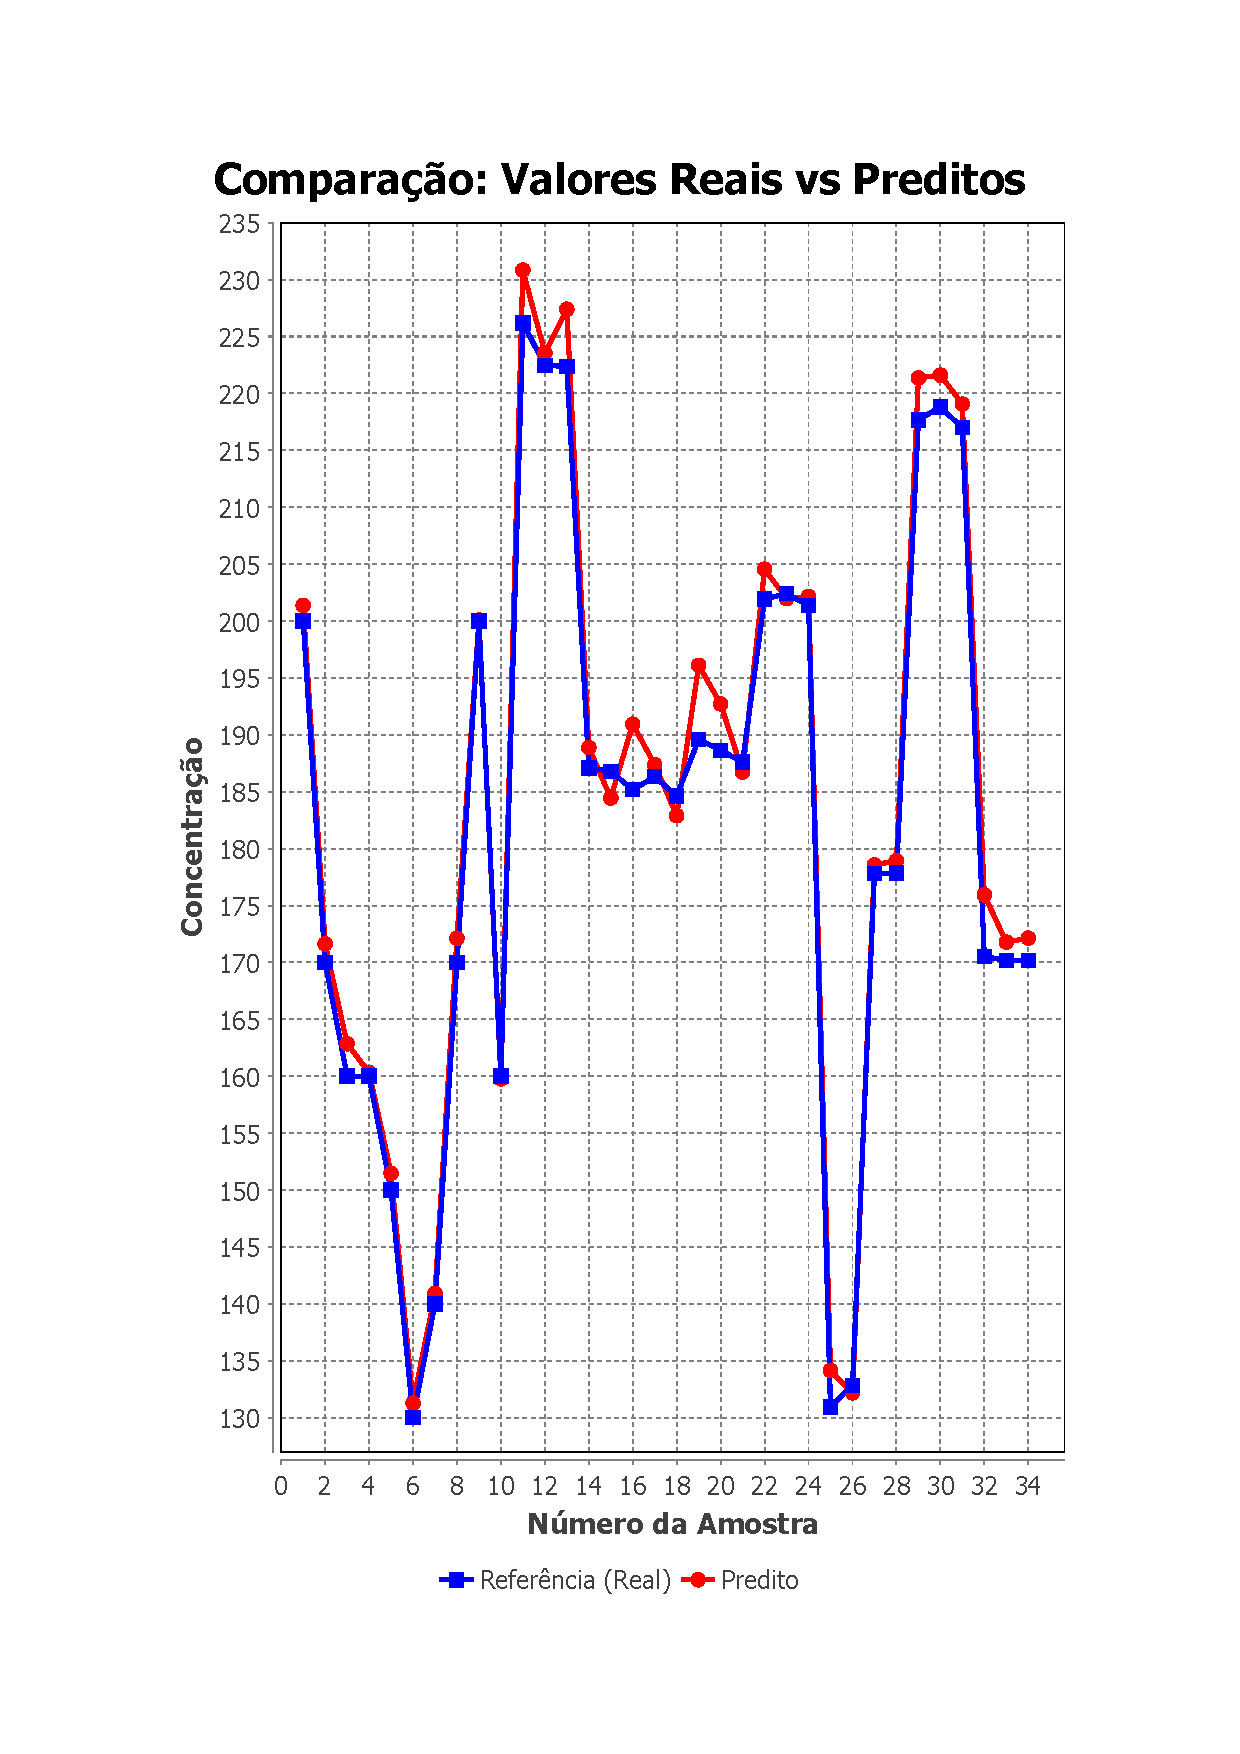
\includepdf[pages=-, scale=0.5]{./outros/fig/BootStrapRMSEPFe.pdf}  % Inclui todas as páginas
%--------------------------------------

\begin{comment}
%--------------------------------------
\begin{figure}[htbp]
\centering
\begin{subfigure}{0.48\textwidth}%{0.48\textwidth}
\centering
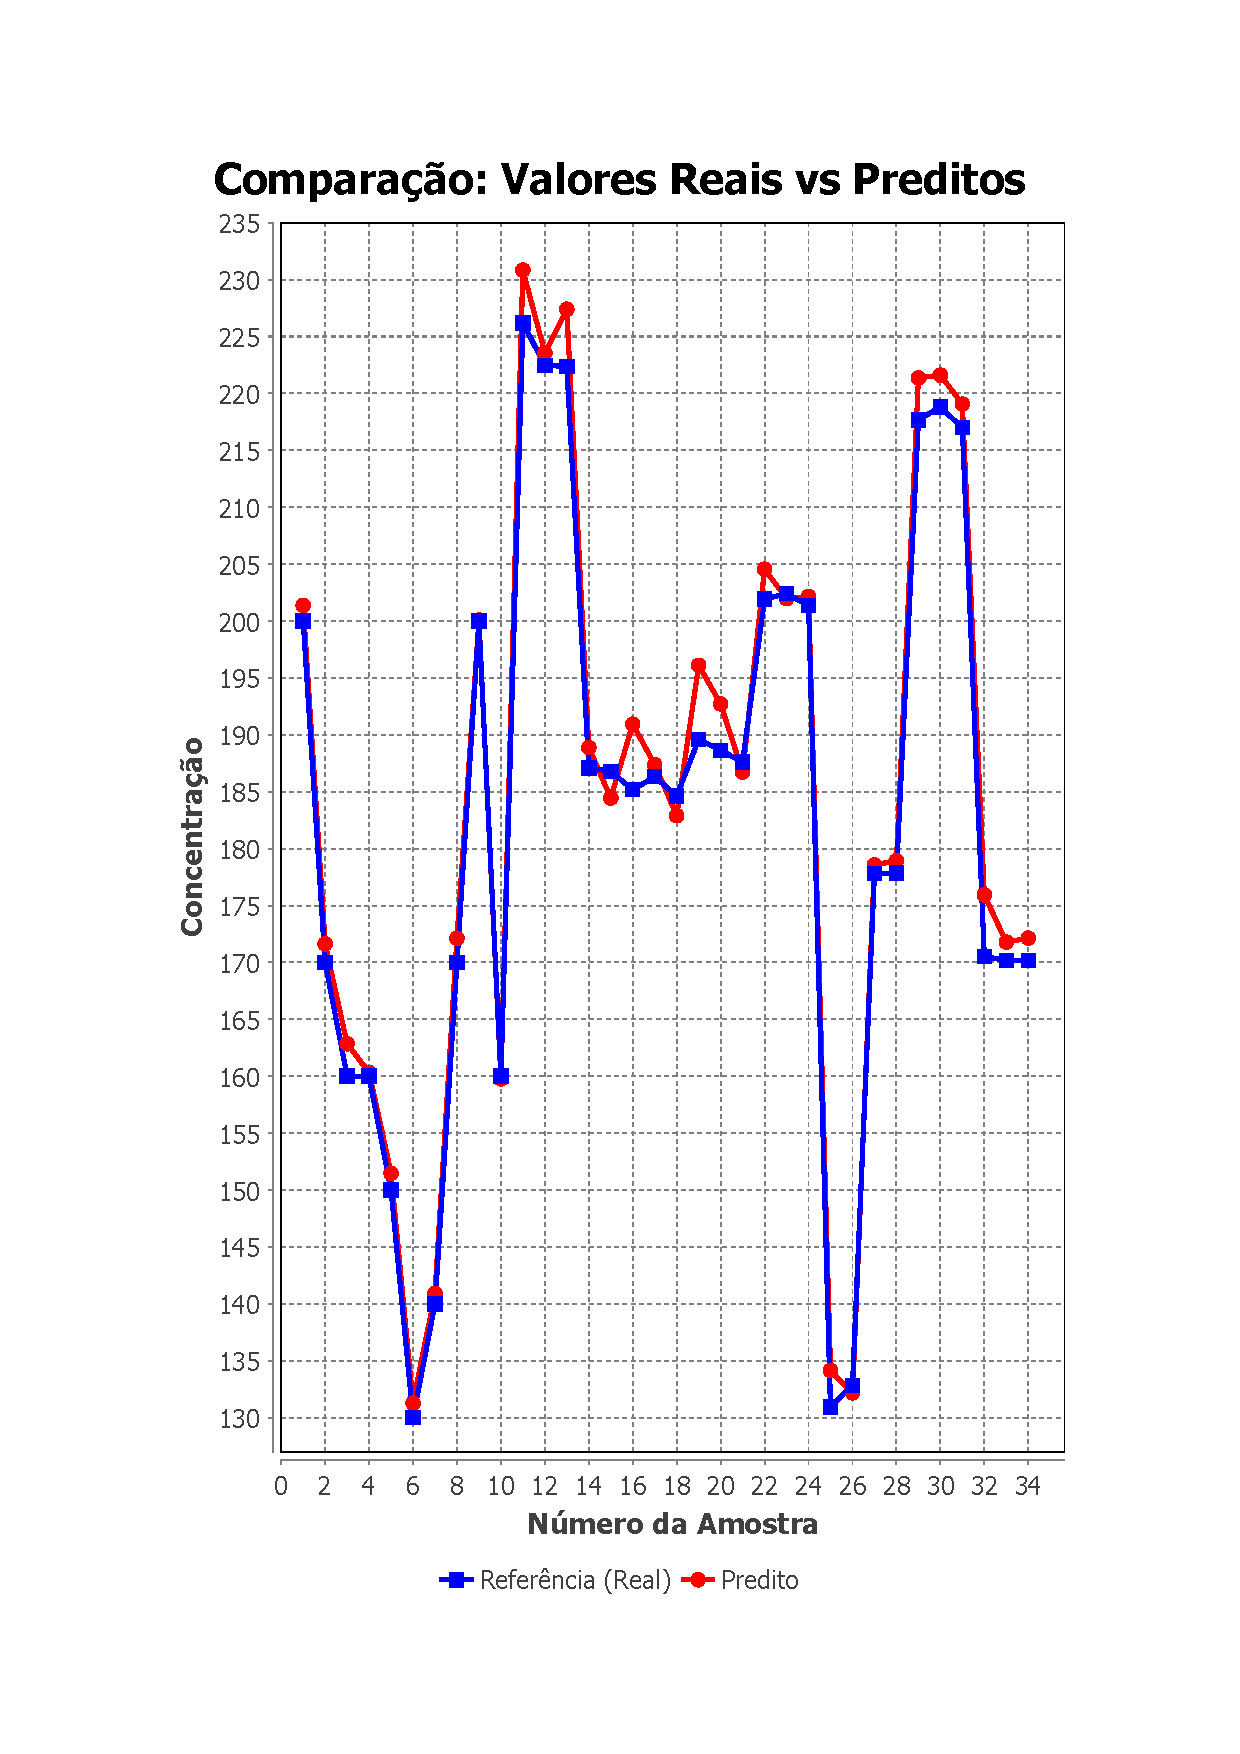
\includegraphics[width=10cm, height=10cm, keepaspectratio]{./outros/fig/BootStrapRMSEPFe.pdf}  % Inclui todas as páginas
\caption{Legenda da figura esquerda}
\label{fig:esquerda}
\end{subfigure}
\hfill
\begin{subfigure}{0.48\textwidth}
\centering
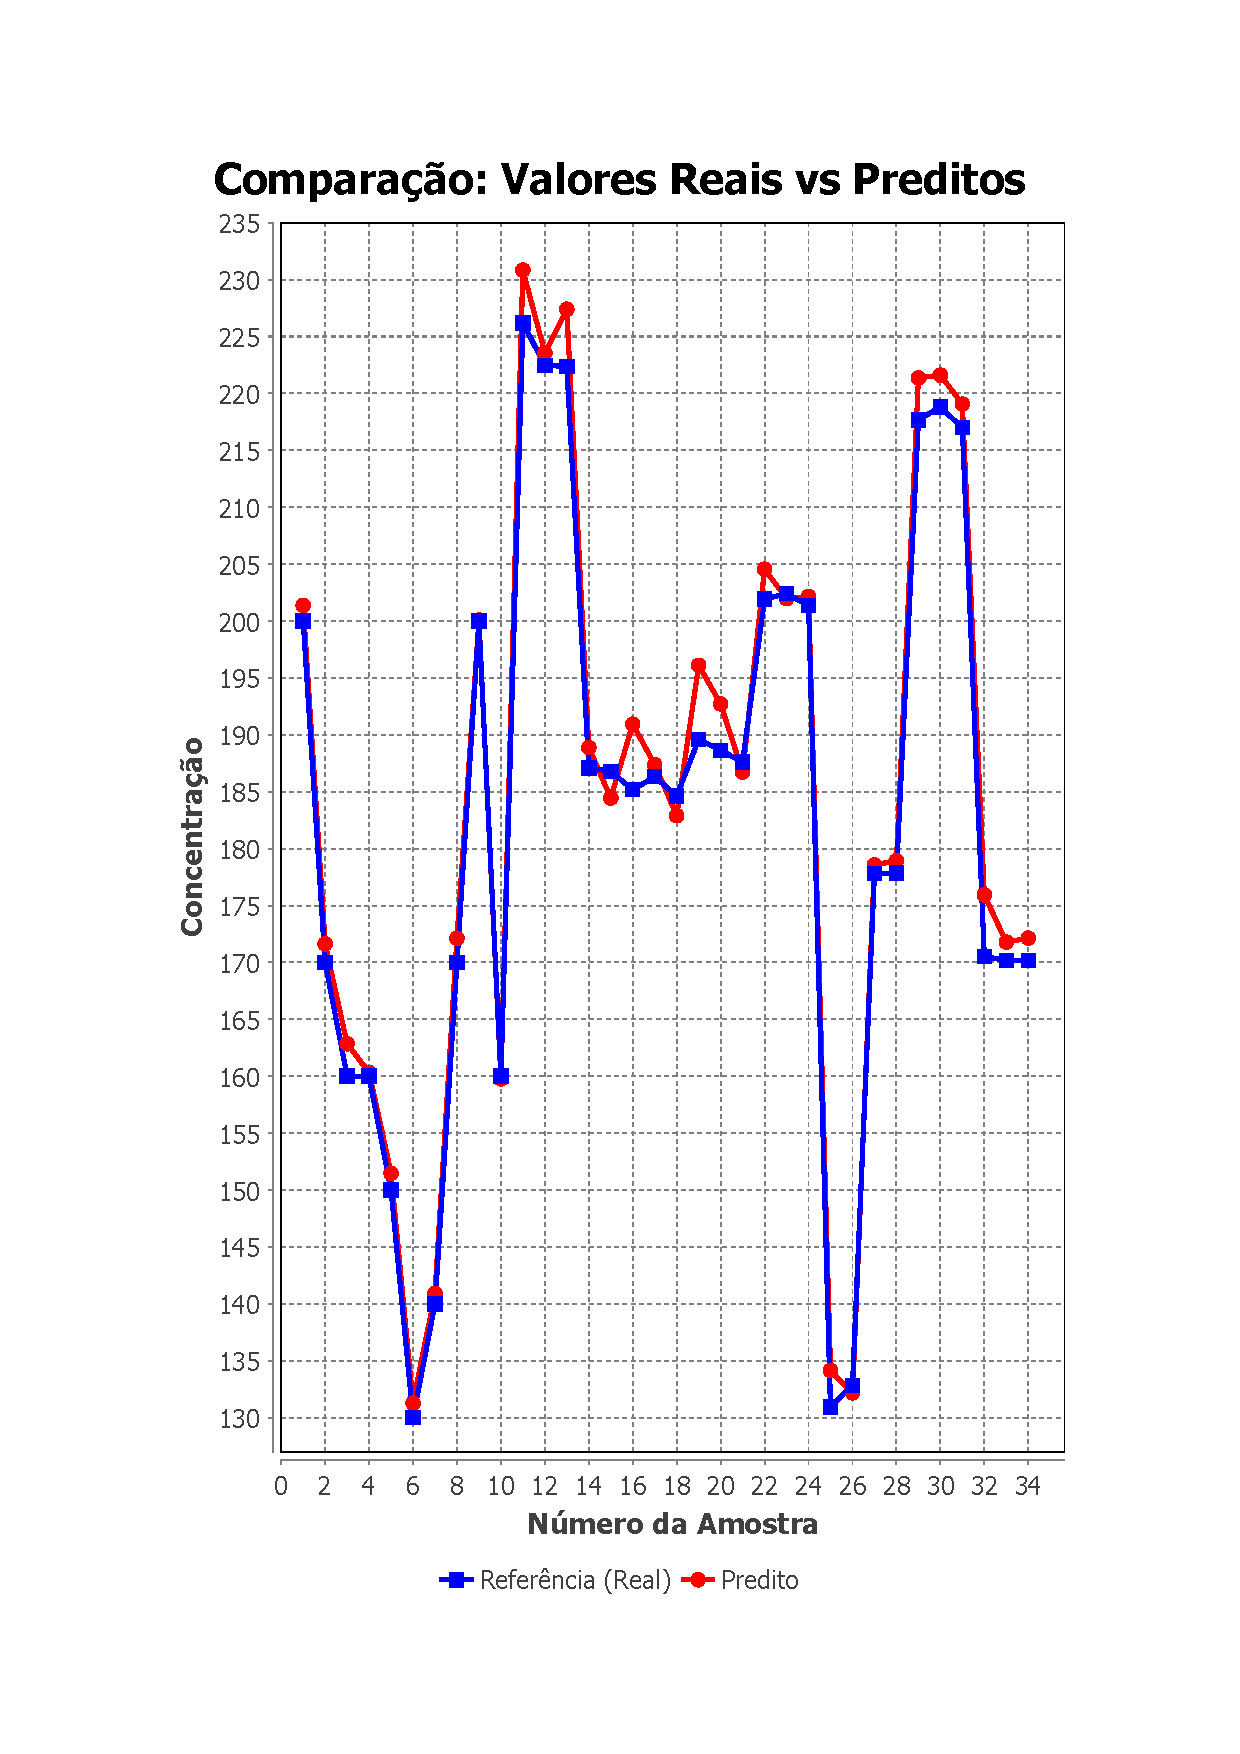
\includegraphics[width=10cm, height=10cm, keepaspectratio]{./outros/fig/BootStrapRMSEPFe.pdf}  % Inclui todas as páginas
\caption{Legenda da figura direita}
\label{fig:direita}
\end{subfigure}
\caption{Legenda geral para as duas figuras}
\label{fig:duas_sub}
\end{figure}

%--------------------------------------
\end{comment}

\begin{comment}

\begin{figure}[htbp]
\centering
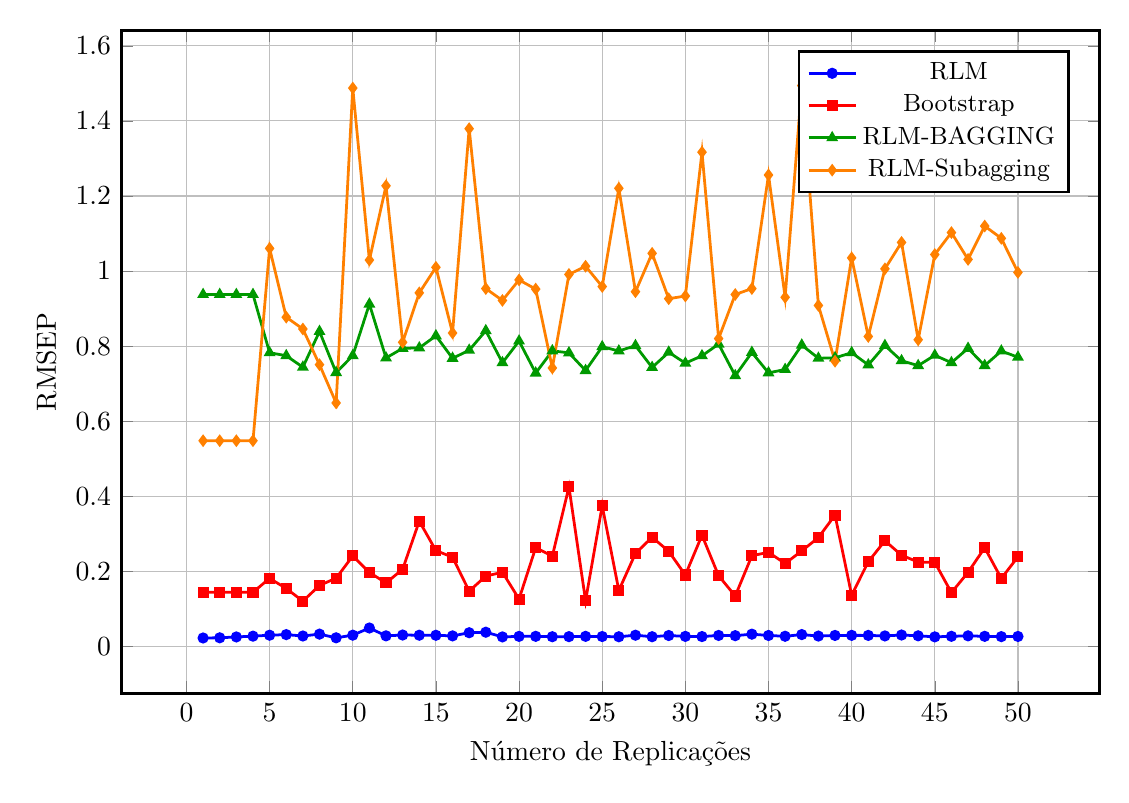
\begin{tikzpicture}
\begin{axis}[
    width=14cm,
    height=10cm,
    xlabel={Número de Replicações},
    ylabel={RMSEP},
    legend pos=north east,
    grid=major,
    legend style={font=\small},
    mark size=1.5pt,
    line width=1pt,
]

% RLM (primeira coluna)
\addplot[color=blue, mark=*, mark options={solid}] coordinates {
(1, 0.0226) (2, 0.0231) (3, 0.0254) (4, 0.0275) (5, 0.0300) (6, 0.0316) (7, 0.0279) (8, 0.0329) (9, 0.0231) (10, 0.0301)
(11, 0.0492) (12, 0.0283) (13, 0.0305) (14, 0.0300) (15, 0.0298) (16, 0.0282) (17, 0.0366) (18, 0.0380) (19, 0.0255) (20, 0.0269)
(21, 0.0270) (22, 0.0260) (23, 0.0262) (24, 0.0270) (25, 0.0265) (26, 0.0259) (27, 0.0300) (28, 0.0260) (29, 0.0292) (30, 0.0269)
(31, 0.0264) (32, 0.0294) (33, 0.0288) (34, 0.0328) (35, 0.0293) (36, 0.0272) (37, 0.0317) (38, 0.0277) (39, 0.0294) (40, 0.0296)
(41, 0.0295) (42, 0.0281) (43, 0.0305) (44, 0.0284) (45, 0.0256) (46, 0.0271) (47, 0.0283) (48, 0.0270) (49, 0.0262) (50, 0.0267)
};

% Bootstrap (segunda coluna)
\addplot[color=red, mark=square*, mark options={solid}] coordinates {
(1, 0.1445) (2, 0.1445) (3, 0.1445) (4, 0.1445) (5, 0.1815) (6, 0.1545) (7, 0.1207) (8, 0.1627) (9, 0.1819) (10, 0.2412)
(11, 0.1972) (12, 0.1693) (13, 0.2058) (14, 0.3339) (15, 0.2554) (16, 0.2378) (17, 0.1474) (18, 0.1875) (19, 0.1977) (20, 0.1263)
(21, 0.2633) (22, 0.2405) (23, 0.4251) (24, 0.1218) (25, 0.3748) (26, 0.1493) (27, 0.2478) (28, 0.2910) (29, 0.2535) (30, 0.1904)
(31, 0.2963) (32, 0.1884) (33, 0.1345) (34, 0.2417) (35, 0.2509) (36, 0.2210) (37, 0.2546) (38, 0.2901) (39, 0.3500) (40, 0.1367)
(41, 0.2256) (42, 0.2816) (43, 0.2431) (44, 0.2248) (45, 0.2240) (46, 0.1434) (47, 0.1976) (48, 0.2630) (49, 0.1811) (50, 0.2389)
};

% RLM-BAGGING (terceira coluna)
\addplot[color=green!60!black, mark=triangle*, mark options={solid}] coordinates {
(1, 0.9375) (2, 0.9375) (3, 0.9375) (4, 0.9375) (5, 0.7825) (6, 0.7745) (7, 0.7439) (8, 0.8391) (9, 0.7296) (10, 0.7746)
(11, 0.9120) (12, 0.7685) (13, 0.7942) (14, 0.7953) (15, 0.8275) (16, 0.7676) (17, 0.7890) (18, 0.8411) (19, 0.7558) (20, 0.8136)
(21, 0.7283) (22, 0.7875) (23, 0.7821) (24, 0.7350) (25, 0.7984) (26, 0.7871) (27, 0.8013) (28, 0.7432) (29, 0.7837) (30, 0.7546)
(31, 0.7743) (32, 0.8055) (33, 0.7212) (34, 0.7833) (35, 0.7288) (36, 0.7378) (37, 0.8027) (38, 0.7678) (39, 0.7688) (40, 0.7826)
(41, 0.7500) (42, 0.8016) (43, 0.7611) (44, 0.7481) (45, 0.7757) (46, 0.7560) (47, 0.7941) (48, 0.7482) (49, 0.7870) (50, 0.7705)
};

% RLM-Subagging (quarta coluna)
\addplot[color=orange, mark=diamond*, mark options={solid}] coordinates {
(1, 0.5481) (2, 0.5481) (3, 0.5481) (4, 0.5481) (5, 1.0603) (6, 0.8772) (7, 0.8456) (8, 0.7506) (9, 0.6487) (10, 1.4875)
(11, 1.0293) (12, 1.2272) (13, 0.8103) (14, 0.9419) (15, 1.0099) (16, 0.8350) (17, 1.3792) (18, 0.9533) (19, 0.9217) (20, 0.9764)
(21, 0.9519) (22, 0.7419) (23, 0.9910) (24, 1.0128) (25, 0.9587) (26, 1.2205) (27, 0.9450) (28, 1.0472) (29, 0.9263) (30, 0.9336)
(31, 1.3167) (32, 0.8202) (33, 0.9376) (34, 0.9533) (35, 1.2558) (36, 0.9301) (37, 1.4940) (38, 0.9084) (39, 0.7599) (40, 1.0352)
(41, 0.8257) (42, 1.0059) (43, 1.0763) (44, 0.8170) (45, 1.0441) (46, 1.1025) (47, 1.0310) (48, 1.1199) (49, 1.0872) (50, 0.9964)
};

\legend{RLM, Bootstrap, RLM-BAGGING, RLM-Subagging}
\end{axis}
\end{tikzpicture}
\caption{RMSEP em função do número de replicações para diferentes técnicas de regressão.}
\label{fig:rmsep}
\end{figure}




\begin{figure}[htbp]
\centering

% Subplot (a) - RLM
\begin{subfigure}[b]{0.48\textwidth}
\centering
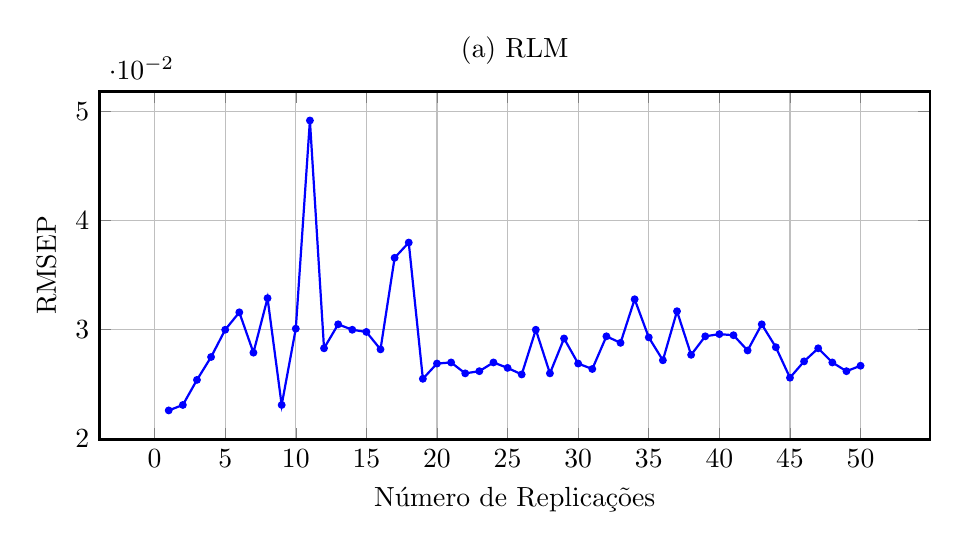
\begin{tikzpicture}
\begin{axis}[
    width=\textwidth,
    height=6cm,
    xlabel={Número de Replicações},
    ylabel={RMSEP},
    title={(a) RLM},
    grid=major,
    mark size=1pt,
    line width=0.8pt,
]
\addplot[color=blue, mark=*, mark options={solid}] coordinates {
(1, 0.0226) (2, 0.0231) (3, 0.0254) (4, 0.0275) (5, 0.0300) (6, 0.0316) (7, 0.0279) (8, 0.0329) (9, 0.0231) (10, 0.0301)
(11, 0.0492) (12, 0.0283) (13, 0.0305) (14, 0.0300) (15, 0.0298) (16, 0.0282) (17, 0.0366) (18, 0.0380) (19, 0.0255) (20, 0.0269)
(21, 0.0270) (22, 0.0260) (23, 0.0262) (24, 0.0270) (25, 0.0265) (26, 0.0259) (27, 0.0300) (28, 0.0260) (29, 0.0292) (30, 0.0269)
(31, 0.0264) (32, 0.0294) (33, 0.0288) (34, 0.0328) (35, 0.0293) (36, 0.0272) (37, 0.0317) (38, 0.0277) (39, 0.0294) (40, 0.0296)
(41, 0.0295) (42, 0.0281) (43, 0.0305) (44, 0.0284) (45, 0.0256) (46, 0.0271) (47, 0.0283) (48, 0.0270) (49, 0.0262) (50, 0.0267)
};
\end{axis}
\end{tikzpicture}
\caption{Regressão Linear Múltipla}
\end{subfigure}
\hfill
% Subplot (b) - Bootstrap
\begin{subfigure}[b]{0.48\textwidth}
\centering
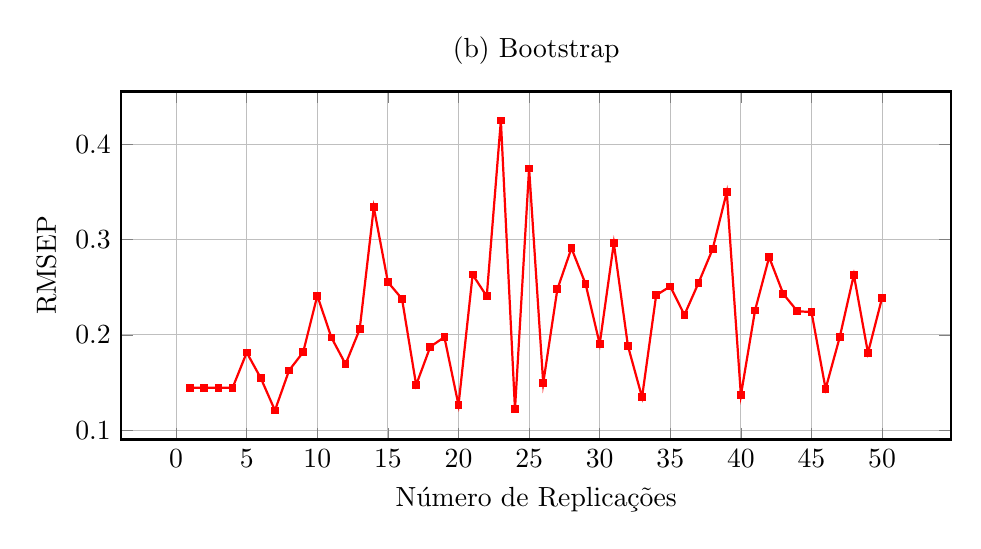
\begin{tikzpicture}
\begin{axis}[
    width=\textwidth,
    height=6cm,
    xlabel={Número de Replicações},
    ylabel={RMSEP},
    title={(b) Bootstrap},
    grid=major,
    mark size=1pt,
    line width=0.8pt,
]
\addplot[color=red, mark=square*, mark options={solid}] coordinates {
(1, 0.1445) (2, 0.1445) (3, 0.1445) (4, 0.1445) (5, 0.1815) (6, 0.1545) (7, 0.1207) (8, 0.1627) (9, 0.1819) (10, 0.2412)
(11, 0.1972) (12, 0.1693) (13, 0.2058) (14, 0.3339) (15, 0.2554) (16, 0.2378) (17, 0.1474) (18, 0.1875) (19, 0.1977) (20, 0.1263)
(21, 0.2633) (22, 0.2405) (23, 0.4251) (24, 0.1218) (25, 0.3748) (26, 0.1493) (27, 0.2478) (28, 0.2910) (29, 0.2535) (30, 0.1904)
(31, 0.2963) (32, 0.1884) (33, 0.1345) (34, 0.2417) (35, 0.2509) (36, 0.2210) (37, 0.2546) (38, 0.2901) (39, 0.3500) (40, 0.1367)
(41, 0.2256) (42, 0.2816) (43, 0.2431) (44, 0.2248) (45, 0.2240) (46, 0.1434) (47, 0.1976) (48, 0.2630) (49, 0.1811) (50, 0.2389)
};
\end{axis}
\end{tikzpicture}
\caption{Bootstrap}
\end{subfigure}

\vspace{0.5cm}

% Subplot (c) - RLM-BAGGING
\begin{subfigure}[b]{0.48\textwidth}
\centering
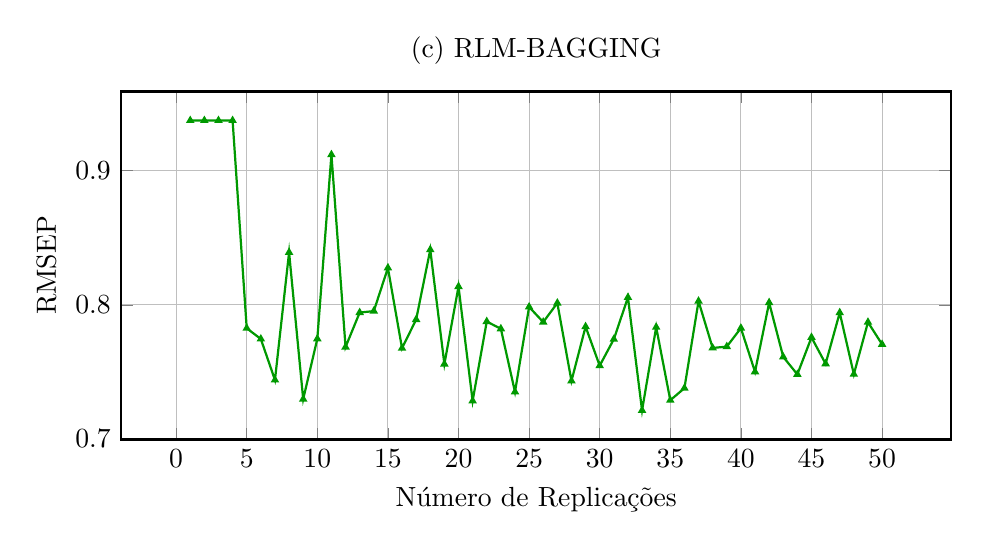
\begin{tikzpicture}
\begin{axis}[
    width=\textwidth,
    height=6cm,
    xlabel={Número de Replicações},
    ylabel={RMSEP},
    title={(c) RLM-BAGGING},
    grid=major,
    mark size=1pt,
    line width=0.8pt,
]
\addplot[color=green!60!black, mark=triangle*, mark options={solid}] coordinates {
(1, 0.9375) (2, 0.9375) (3, 0.9375) (4, 0.9375) (5, 0.7825) (6, 0.7745) (7, 0.7439) (8, 0.8391) (9, 0.7296) (10, 0.7746)
(11, 0.9120) (12, 0.7685) (13, 0.7942) (14, 0.7953) (15, 0.8275) (16, 0.7676) (17, 0.7890) (18, 0.8411) (19, 0.7558) (20, 0.8136)
(21, 0.7283) (22, 0.7875) (23, 0.7821) (24, 0.7350) (25, 0.7984) (26, 0.7871) (27, 0.8013) (28, 0.7432) (29, 0.7837) (30, 0.7546)
(31, 0.7743) (32, 0.8055) (33, 0.7212) (34, 0.7833) (35, 0.7288) (36, 0.7378) (37, 0.8027) (38, 0.7678) (39, 0.7688) (40, 0.7826)
(41, 0.7500) (42, 0.8016) (43, 0.7611) (44, 0.7481) (45, 0.7757) (46, 0.7560) (47, 0.7941) (48, 0.7482) (49, 0.7870) (50, 0.7705)
};
\end{axis}
\end{tikzpicture}
\caption{RLM com Bagging}
\end{subfigure}
\hfill
% Subplot (d) - RLM-Subagging
\begin{subfigure}[b]{0.48\textwidth}
\centering
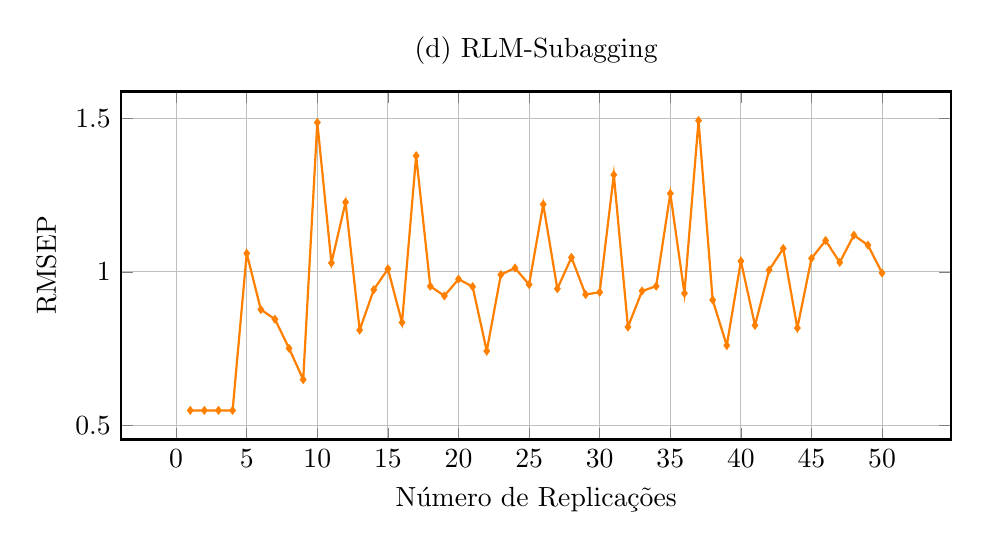
\begin{tikzpicture}
\begin{axis}[
    width=\textwidth,
    height=6cm,
    xlabel={Número de Replicações},
    ylabel={RMSEP},
    title={(d) RLM-Subagging},
    grid=major,
    mark size=1pt,
    line width=0.8pt,
]
\addplot[color=orange, mark=diamond*, mark options={solid}] coordinates {
(1, 0.5481) (2, 0.5481) (3, 0.5481) (4, 0.5481) (5, 1.0603) (6, 0.8772) (7, 0.8456) (8, 0.7506) (9, 0.6487) (10, 1.4875)
(11, 1.0293) (12, 1.2272) (13, 0.8103) (14, 0.9419) (15, 1.0099) (16, 0.8350) (17, 1.3792) (18, 0.9533) (19, 0.9217) (20, 0.9764)
(21, 0.9519) (22, 0.7419) (23, 0.9910) (24, 1.0128) (25, 0.9587) (26, 1.2205) (27, 0.9450) (28, 1.0472) (29, 0.9263) (30, 0.9336)
(31, 1.3167) (32, 0.8202) (33, 0.9376) (34, 0.9533) (35, 1.2558) (36, 0.9301) (37, 1.4940) (38, 0.9084) (39, 0.7599) (40, 1.0352)
(41, 0.8257) (42, 1.0059) (43, 1.0763) (44, 0.8170) (45, 1.0441) (46, 1.1025) (47, 1.0310) (48, 1.1199) (49, 1.0872) (50, 0.9964)
};
\end{axis}
\end{tikzpicture}
\caption{RLM com Subagging}
\end{subfigure}

\caption{RMSEP em função do número de replicações para diferentes técnicas de regressão.}
\label{fig:rmsep_completo}
\end{figure}

\end{comment}


\begin{comment}

\begin{center}
\textbf{\textit{Bagging (Bootstrap Aggregating)}}
\end{center}
\resizebox{0.90\textwidth}{!}{ % Ajuste a largura aqui (0.95 = 95% da largura da página)
\begin{tikzpicture}[
  node distance=1.5cm and 2cm,
  every node/.style={draw, font=\small, align=center},
  bootstrap/.style={ellipse, draw},
  model/.style={rectangle, draw},
  arrow/.style={-{Stealth}, thick}
]

% Nodes
\node (data) [rectangle] {Conjunto\\ de Dados\\Calibração};

\node (sample1) [bootstrap, right=of data, yshift=2cm] {Bootstrap\\Amostra $1$};
\node (sample2) [bootstrap, right=of data] {Bootstrap\\Amostra $2$};
\node (samplen) [bootstrap, right=of data, yshift=-2cm] {Bootstrap\\Amostra $n$};

\node (model1) [model, right=of sample1] {Modelo $1$};
\node (model2) [model, right=of sample2] {Modelo $2$};
\node (modeln) [model, right=of samplen] {Modelo $n$};

\node (avg) [rectangle, right=of model2, xshift=2cm] {Média\\Modelo};

% Arrows
\draw[arrow] (data) -- (sample1);
\draw[arrow] (data) -- (sample2);
\draw[arrow] (data) -- (samplen);

\draw[arrow] (sample1) -- (model1);
\draw[arrow] (sample2) -- (model2);
\draw[arrow] (samplen) -- (modeln);

\draw[arrow] (model1) -- (avg);
\draw[arrow] (model2) -- (avg);
\draw[arrow] (modeln) -- (avg);

% Dots
\node at ($(sample2)!0.5!(samplen)$) {\vdots};
\node at ($(model2)!0.5!(modeln)$) {\vdots};

\end{tikzpicture}
}
%-------------------------------------------------------------------------------------



\begin{center}
\textbf{Subagging (Subsample Aggregating)}
\end{center}

% Resizebox para controlar o tamanho do diagrama
\resizebox{0.95\textwidth}{!}{ % Ajuste a largura aqui (0.95 = 95% da largura da página)
\begin{tikzpicture}[
  node distance=1.5cm and 2cm,
  every node/.style={draw, font=\small, align=center},
  subsample/.style={ellipse, draw},
  model/.style={rectangle, draw},
  arrow/.style={-{Stealth}, thick}
]

% Nós
\node (data) [rectangle] {Conjunto \\de Dados\\Calibração};

\node (sub1) [subsample, right=of data, yshift=2.5cm] {Subamostra 1};
\node (sub2) [subsample, right=of data] {Subamostra 2};
\node (subn) [subsample, right=of data, yshift=-2.5cm] {Subamostra n};

\node (model1) [model, right=of sub1] {X $\rightarrow$ Modelo 1};
\node (model2) [model, right=of sub2] {X $\rightarrow$ Modelo 2};
\node (modeln) [model, right=of subn] {X $\rightarrow$ Modelo n};

\node (avg) [rectangle, right=of model2, xshift=2cm] {Média $\rightarrow$ Y};

% Setas
\draw[arrow] (data) -- (sub1);
\draw[arrow] (data) -- (sub2);
\draw[arrow] (data) -- (subn);

\draw[arrow] (sub1) -- (model1);
\draw[arrow] (sub2) -- (model2);
\draw[arrow] (subn) -- (modeln);

\draw[arrow] (model1) -- (avg);
\draw[arrow] (model2) -- (avg);
\draw[arrow] (modeln) -- (avg);

% Pontos de continuação
\node at ($(sub2)!0.5!(subn)$) {\vdots};
\node at ($(model2)!0.5!(modeln)$) {\vdots};

\end{tikzpicture}
} % Fim do resizebox

%------------------------------------------------------------------------------

%-------------------------------------------------------------------
\newpage

\begin{center}
\textbf{RLM com Bagging e Avaliação com RMSEP}
\end{center}

\resizebox{0.90\textwidth}{!}{
\begin{tikzpicture}[
  node distance=1.5cm and 2.5cm,
  every node/.style={draw, font=\small, align=center},
  data/.style={rectangle, draw},
  sample/.style={ellipse, draw},
  model/.style={rectangle, draw},
  arrow/.style={-{Stealth}, thick}
]

% Etapas iniciais
\node (dataset) [data] {Conjunto\\ de Dados};
\node (split) [data, right=of dataset] {Divisão\\60\% Calibração\\40\% Teste};
\node (bagging) [data, right=of split] {Bagging};

% Amostras bootstrap (mais abaixo)
\node (bs1) [sample, below=of bagging, yshift=-1cm] {Bootstrap 1};
\node (bs2) [sample, below=of bs1] {Bootstrap 2};
\node (bsn) [sample, below=of bs2] {Bootstrap n};

% Modelos RLM
\node (model1) [model, right=of bs1] {RLM 1};
\node (model2) [model, right=of bs2] {RLM 2};
\node (modeln) [model, right=of bsn] {RLM n};

% Agregação de previsões
\node (pred) [data, right=of model2, xshift=2cm] {Agregação\\de Previsões};

% Teste e RMSEP
\node (test) [data, below=of split, yshift=-6.5cm] {40\% Teste};
\node (rmsep) [data, right=of test, xshift=6.5cm] {RMSEP};

% Conexões principais
\draw[arrow] (dataset) -- (split);
\draw[arrow] (split) -- (bagging);

\draw[arrow] (bagging) -- (bs1);
%\draw[arrow] (bagging) -- (bs2);
%\draw[arrow] (bagging) -- (bsn);

\draw[arrow] (bs1) -- (model1);
\draw[arrow] (bs2) -- (model2);
\draw[arrow] (bsn) -- (modeln);

\draw[arrow] (model1) -- (pred);
\draw[arrow] (model2) -- (pred);
\draw[arrow] (modeln) -- (pred);

\draw[arrow] (test) -- (rmsep);
\draw[arrow] (pred) -- (rmsep);

% Pontos de continuação
\node at ($(bs2)!0.5!(bsn)$) {\vdots};
\node at ($(model2)!0.5!(modeln)$) {\vdots};

\end{tikzpicture}
}

%--------------------------------------------------------------------------


\begin{center}
\textbf{RLM com Subagging e Avaliação com RMSEP}
\end{center}

\resizebox{0.90\textwidth}{!}{
\begin{tikzpicture}[
  node distance=1.5cm and 2.5cm,
  every node/.style={draw, font=\small, align=center},
  data/.style={rectangle, draw},
  sample/.style={ellipse, draw},
  model/.style={rectangle, draw},
  arrow/.style={-{Stealth}, thick}
]

% Etapas iniciais
\node (dataset) [data] {Conjunto\\ de Dados};
\node (split) [data, right=of dataset] {Divisão\\60\% Calibração\\40\% Teste};
\node (bagging) [data, right=of split] {Subagging};

% Amostras bootstrap (mais abaixo)
\node (bs1) [sample, below=of bagging, yshift=-1cm] {Subamostra 1};
\node (bs2) [sample, below=of bs1] {Subamostra 2};
\node (bsn) [sample, below=of bs2] {Subamostra n};

% Modelos RLM
\node (model1) [model, right=of bs1] {RLM 1};
\node (model2) [model, right=of bs2] {RLM 2};
\node (modeln) [model, right=of bsn] {RLM n};

% Agregação de previsões
\node (pred) [data, right=of model2, xshift=2cm] {Agregação\\de Previsões};

% Teste e RMSEP
\node (test) [data, below=of split, yshift=-6.5cm] {40\% Teste};
\node (rmsep) [data, right=of test, xshift=6.5cm] {RMSEP};

% Conexões principais
\draw[arrow] (dataset) -- (split);
\draw[arrow] (split) -- (bagging);

\draw[arrow] (bagging) -- (bs1);
%\draw[arrow] (bagging) -- (bs2);
%\draw[arrow] (bagging) -- (bsn);

\draw[arrow] (bs1) -- (model1);
\draw[arrow] (bs2) -- (model2);
\draw[arrow] (bsn) -- (modeln);

\draw[arrow] (model1) -- (pred);
\draw[arrow] (model2) -- (pred);
\draw[arrow] (modeln) -- (pred);

\draw[arrow] (test) -- (rmsep);
\draw[arrow] (pred) -- (rmsep);

% Pontos de continuação
\node at ($(bs2)!0.5!(bsn)$) {\vdots};
\node at ($(model2)!0.5!(modeln)$) {\vdots};

\end{tikzpicture}
}

%--------------------------------------------------------------------------
\end{comment}

%---------------------------------\documentclass[border=5pt]{standalone}


\begin{comment}
\begin{figure}[htbp]
\centering
\caption{Espectros médios dos analitos analisados.}
\label{fig:tempo}
\resizebox{0.50\columnwidth}{!}{%
\begin{tikzpicture}
\begin{axis}[
    width=12cm,
    height=9cm,
    %title={\textbf{Espectros Médios - 5 Elementos}},
    title style={font=\large},
    xlabel={Comprimento de Onda (nm)},
    ylabel={Intensidades},
    xlabel style={font=\normalsize},
    ylabel style={font=\normalsize},
    xmin=200, xmax=800,
    ymin=0, ymax=3000,
    grid=major,
    grid style={line width=0.3pt, draw=gray!40},
    legend pos=north east,
    legend style={
        font=\small,
        cells={anchor=west},
        draw=black,
        fill=white,
        line width=0.5pt
    },
    line width=1.5pt,
    tick label style={font=\small},
    axis background/.style={fill=white},
    axis lines=left,
    every axis plot/.append style={no marks}
]

% Espectro do Fe (verde)
\addplot[verde, line width=1.5pt] table[
    x expr=200+\coordindex*(600/722),
    y index=0,
    header=false
] {G:/TecnicasDeReamostragem/Projeto_Integrador_III_Final/outros/prog/dados_Fe.txt};
\addlegendentry{Fe}

% Espectro do Cr (vermelho)
\addplot[vermelho, line width=1.5pt] table[
    x expr=200+\coordindex*(600/722),
    y index=0,
    header=false
] {G:/TecnicasDeReamostragem/Projeto_Integrador_III_Final/outros/prog/dados_Cr.txt};
\addlegendentry{Cr}

% Espectro do Mn (azul)
\addplot[azul, line width=1.5pt] table[
    x expr=200+\coordindex*(600/722),
    y index=0,
    header=false
] {G:/TecnicasDeReamostragem/Projeto_Integrador_III_Final/outros/prog/dados_Mn.txt};
\addlegendentry{Mn}

% Espectro do Ni (magenta)
\addplot[magenta, line width=1.5pt] table[
    x expr=200+\coordindex*(600/722),
    y index=0,
    header=false
] {G:/TecnicasDeReamostragem/Projeto_Integrador_III_Final/outros/prog/dados_Ni.txt};
\addlegendentry{Ni}

% Espectro do Mo (ciano)
\addplot[ciano, line width=1.5pt] table[
    x expr=200+\coordindex*(600/722),
    y index=0,
    header=false
] {G:/TecnicasDeReamostragem/Projeto_Integrador_III_Final/outros/prog/dados_Mo.txt};
\addlegendentry{Mo}

\end{axis}
\end{tikzpicture}
}%Fim raisebox
\legend{Fonte: elaborado pelo autor.}
\end{figure}
\end{comment}


